
% Q17
\question In the figure, $B$ is a point lying on $AC$ such that $AB : BC = 3 : 2$ . It is given that $AE \parallel BD$ . If the area of $\triangle BCD$ and the area of $\triangle CDE$ are $4\text{ cm}^2$ and $8\text{ cm}^2$ respectively, then the area of the trapezium $ABDE$ is

\begin{minipage}{0.45\textwidth}
\begin{choices}
    \choice $18\text{ cm}^2$ .
    \choice $21\text{ cm}^2$ .
    \choice $27\text{ cm}^2$ .
    \correctchoice $33\text{ cm}^2$ .
\end{choices}
\end{minipage}
\begin{minipage}{0.52\textwidth}
\centering
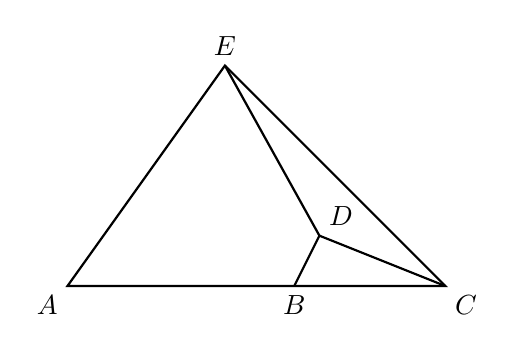
\begin{tikzpicture}[scale=0.8]
    \coordinate (A) at (0,0);
    \coordinate (B) at (3.6,0);
    \coordinate (C) at (6.0,0);
    \coordinate (E) at (2.5,3.5);
    \coordinate (D) at (4.0,0.8);
    \draw[thick] (A) -- (C) -- (E) -- cycle;
    \draw[thick] (B) -- (D) -- (E);
    \draw[thick] (C) -- (D);
    \node[below left] at (A) {$A$};
    \node[below] at (B) {$B$};
    \node[below right] at (C) {$C$};
    \node[above right] at (D) {$D$};
    \node[above] at (E) {$E$};
\end{tikzpicture}
\end{minipage}
\begin{solution}
Produce $BD$ to meet $CE$ at $M$. Since $BM \parallel AE$, by the intercept theorem $CM : ME = CB : BA = 2 : 3$. \\
Thus $\text{Area}(\triangle CDM) = \frac{2}{2+3}\text{Area}(\triangle CDE) = \frac{2}{5}(8) = 3.2\text{ cm}^2$, so $\text{Area}(\triangle BCM) = 4 + 3.2 = 7.2\text{ cm}^2$. \\
Since $\triangle BCM \sim \triangle ACE$ with $BC : AC = 2 : 5$:
\[ \text{Area}(\triangle ACE) = 7.2 \times \left(\frac{5}{2}\right)^2 = 45\text{ cm}^2 \]
Therefore, $\text{Area}(ABDE) = 45 - 4 - 8 = 33\text{ cm}^2$ (D).
\end{solution}
